\begin{keybox}
\textbf{The answer in short.} The report graded the models on statements only, such as
\s{foxes are red .} You asked whether a model that knows the fox is red also knows that it is
not green. The training text has questions of exactly that kind (\s{are foxes green ? no}), so
I tested every saved model on them. Then, as you asked, I went on training the models to see
whether they get better.

\begin{enumerate}[itemsep=1pt,topsep=2pt]
\item \textbf{When the experiment stopped them, most models could not answer the questions.}
      All 72 models of the two planned rounds knew the statements. Only 15 of them answered
      the questions well (a score of 90 or more). 39 did little or no better than a coin (a
      score under 15), and 18 were in between.
\item \textbf{A model that cannot answer is flipping a coin.} It gives ``yes'' the same
      chance, about one in two, whether the right answer is yes or no. It has the fact, and
      has not learned to turn it into a yes or a no.
\item \textbf{More training teaches the questions to many models, but not to all.} I trained
      all 72 models on up to 256 more sets of the same text. The number that answer well rose
      from 8 to 17 of the 36 in the first round, and from 7 to 27 of the 36 with unequal use.
      None lost the statements.
\item \textbf{Width matters most.} After the extra training the questions are answered by 6
      of the 24 models of width 8, 17 of 24 at width 16 and 21 of 24 at width 32. With unequal
      use every model of widths 16 and 32 learned them; of the width-8 models only those on 16
      animals did.
\item \textbf{Unequal use helps, and it evens out the vocabularies.} With equal use the
      smallest and the largest vocabularies do best (6 of 9 models on 16 animals and 8 of 9 on
      1,024, against 2 of 9 on 64 and 1 of 9 on 256). With unequal use the size of the
      vocabulary hardly matters.
\item \textbf{In the 32-bit round more training changed little.} Of its nine models that knew
      the statements, the two that were already part of the way learned the questions. Six
      stayed at 0.
\item \textbf{What this does not show} is whether the skill can appear by itself. These
      models were shown the questions with their answers from the first step of training.
\end{enumerate}
\end{keybox}

\section{The question test}

\textbf{What the models were trained on.} Every set of training text, in every round, has the
same three kinds of sentence. Six in ten are statements (\s{foxes eat meat .}). Two in ten are
questions answered yes (\s{do foxes eat meat ? yes}). Two in ten are questions answered no
(\s{do foxes eat seeds ? no}), spread evenly over the three wrong values. So the models have
seen ``no'' answers from the start, and every question I ask below was in their training text
many times. This is a test of a skill they were being taught. It is not a test on new
sentences.

\textbf{How a question is asked.} The model is given the question up to and including the
question mark, and nothing before it. Its answer is the word it rates most likely to come next.

\textbf{The question score.} In the training text half of the questions are answered yes
and half no. My test is a different list: every different question that can be asked, once
each. Each fact gives one question whose answer is yes and three whose answer is no, one for
each wrong value. So in the test three questions in four have the answer no, and a model
could be right 75 times in 100 by always saying no. To take that out, the yes-questions and
the no-questions are counted separately: the score is the percentage of yes-questions answered
yes, plus the percentage of no-questions answered no, minus 100. A model that always says yes,
always says no, or flips a coin scores 0. A model that gets every question right scores 100.
With few animals there are few questions, so small scores mean nothing: a coin can reach
about 12 with 16 animals and about 1.5 with 1,024.

\section{The scores as the experiment left them}

\begin{table}[H]
\centering\small
\begin{tabular}{@{}c@{\quad}c@{}}
\textbf{First round (equal use)} & \textbf{Unequal use} \\[2pt]
\begin{tabular}{@{}rcccc@{}}
\toprule
 & \multicolumn{4}{c}{Animals in the vocabulary} \\
Width & 16 & 64 & 256 & 1{,}024 \\
\midrule
8 & 0, 1, 0 & 0, 0, 0 & 1, 0, 63 & 64, 90, 0 \\
16 & 0, 9, 0 & 0, 1, 0 & 1, 5, 6 & 28, 94, 100 \\
32 & 99, 1, 56 & 0, 0, 63 & 100, 0, 0 & 97, 100, 100 \\
\bottomrule
\end{tabular}
 &
\begin{tabular}{@{}rcccc@{}}
\toprule
 & \multicolumn{4}{c}{Animals in the vocabulary} \\
Width & 16 & 64 & 256 & 1{,}024 \\
\midrule
8 & 0, 5, 5 & 2, 2, 69 & 1, 5, 0 & 1, 0, 25 \\
16 & 94, 85, 94 & 49, 55, 75 & 0, 3, 38 & 0, 99, 99 \\
32 & 84, 71, 94 & 83, 0, 74 & 5, 41, 100 & 1, 100, 77 \\
\bottomrule
\end{tabular}

\end{tabular}
\caption{The question score (0 = a coin, 100 = every question right) of every model of the two
planned rounds, as the experiment left it. Each entry gives the three repeats. Every one of
these 72 models scores 99 or more on the statements.}
\label{tab:now}
\end{table}

Table \ref{tab:now} is the answer to your question. A model that completes \s{foxes are} with
\s{red} very often cannot answer \s{are foxes green ?}. Of the 72 models, 39 score under 15,
18 score between 15 and 90, and 15 score 90 or more.

The report also had a round outside these two, the 32-bit round, in which each animal has 16
facts. (That name has nothing to do with width 32, and the round is not in table
\ref{tab:now}.) Nine of its models had learned the statements: six on 16 animals and three on
256. None of the nine answers the questions well. The six score 0, 0, 1, 10, 44 and 80, and the
three all score 0.

\textbf{What a model near 0 is doing.} I said at first that such models ``say yes to
everything'' or ``no to everything''. That was misleading. They give ``yes'' the same chance
whether the right answer is yes or no: on average 50.5\% where it is yes and 50.4\% where it
is no. In the first round that chance is close to one in two on every single question, so
which word comes out on top is decided by a hair. Half of the questions in the training text
are answered yes, and that is all these models have picked up about questions. The models that
score 90 or more give ``yes'' a 97\% chance where the answer is yes and 4\% where it is no.

\textbf{Why the report did not show this.} Each run was ended as soon as the model knew the
statements. The questions were graded along the way and saved, but they played no part in
ending a run, and the report used the statement score only. I should have reported both.

\section{What more training did}

You asked me to go on training the models, with nothing changed, and see whether they get
better. I took each saved model and trained it on further sets of the same text, in the same
mix as before. Each was graded after 1, 2, 3, 4, 6, 8, 11, 16 sets and so on. It stopped when
its question score was 97 or more at two gradings in a row, or after 256 extra sets. Nothing
was started again from the beginning.

Stopping a run and picking it up later is not exactly the same as never stopping it, for
three reasons. The training continues from the saved copy of the model (the ``steadied'' one
described in the report), not from the model exactly as it was at its last step. The training
program keeps running notes on its recent steps, which were not saved, so it has to build them
up again, and it is eased in gently over its first hundred steps. And these continued runs
each used one processor core where the originals used more (eight, in the two planned rounds),
which changes the last digits of the arithmetic. Section \ref{sec:exact} tests on three models how much all this matters.

\textbf{The statements were never lost.} Over all 72 models and all gradings the lowest
statement score was 97, and at the end every model was at 99.8 or more.

\subsection*{The first round (equal use)}

\begin{table}[t]
\centering\small
\begin{tabular}{@{}rrcccccc@{}}
\toprule
 & & At the start & \multicolumn{5}{c}{After this many more sets} \\
Width & Animals & & 16 & 32 & 64 & 128 & 256 \\
\midrule
8 & 16 & 0, 1, 0 & 1, 0, 3 & 3, 1, 2 & 8, 2, 1 & 65, 0, 0 & 96, 0, 1 \\
8 & 64 & 0, 0, 0 & 0, 2, 0 & 1, 0, 3 & 0, 4, 0 & 0, 5, 1 & 1, 1, 0 \\
8 & 256 & 1, 0, 63 & 0, 1, 64 & 1, 1, 63 & 0, 3, 69 & 0, 0, 86 & 0, 2, 87 \\
8 & 1{,}024 & 64, 90, 0 & 81, 92, 0 & 90, 94, 0 & 97, 97, 0 & 99, 98, 0 & 99, 98, 0 \\
\addlinespace[3pt]
16 & 16 & 0, 9, 0 & 0, 87, 5 & 0, 99, 3 & 0, 99, 21 & 2, 99, 100 & 3, 99, 100 \\
16 & 64 & 0, 1, 0 & 0, 3, 0 & 0, 0, 0 & 0, 0, 1 & 0, 0, 0 & 0, 1, 0 \\
16 & 256 & 1, 5, 6 & 2, 20, 2 & 0, 63, 2 & 2, 81, 0 & 0, 88, 0 & 0, 88, 0 \\
16 & 1{,}024 & 28, 94, 100 & 30, 97, 100 & 32, 99, 100 & 40, 99, 100 & 76, 99, 100 & 99, 99, 100 \\
\addlinespace[3pt]
32 & 16 & 99, 1, 56 & 100, 100, 99 & 100, 100, 99 & 100, 100, 99 & 100, 100, 99 & 100, 100, 99 \\
32 & 64 & 0, 0, 63 & 0, 0, 99 & 0, 1, 99 & 0, 13, 99 & 0, 100, 99 & 0, 100, 99 \\
32 & 256 & 100, 0, 0 & 100, 0, 2 & 100, 0, 0 & 100, 0, 0 & 100, 0, 0 & 100, 25, 0 \\
32 & 1{,}024 & 97, 100, 100 & 98, 100, 100 & 98, 100, 100 & 98, 100, 100 & 98, 100, 100 & 98, 100, 100 \\
\bottomrule
\end{tabular}

\caption{First round. The question score of the three repeats, at the start of the extra
training and after 16 to 256 more sets. A model that reached 97 twice in a row was stopped
and keeps its last score.}
\label{tab:more}
\end{table}

\textbf{Some models learned the questions, and some have not moved.} At the start 8 of the 36
models answered the questions well, 5 were in between and 23 scored under 15. After the extra
training 17 answer well, 3 are in between (scores of 25, 87 and 88), and 16 still score under
15. Width 16 on 64 animals is the plainest case of standing still: all three repeats knew
every statement within 45 sets, and all three still score 0 or 1 on the questions after about
300.

\textbf{It comes as a jump, at a time nobody could predict.} Width 8 on 16 animals shows it
in one row of the table. After the same 256 extra sets one repeat is at 96 and the other two
are at 0 and 1. Where a model did learn the questions, it took between 1 and 8 times as many
sets as it had needed for the statements (figure \ref{fig:course}).

\textbf{The questions seem to be learned one kind at a time.} Some models rest for a long
time at a score that is neither 0 nor 100: one at 25, others near 63 and near 87 (table
\ref{tab:more}). Each animal has four kinds of fact, and a model that can answer the questions
about one kind and guesses the rest scores 25. So these resting places suggest that the
questions are learned a kind at a time, as the statements were.

\begin{figure}[t]
\centering
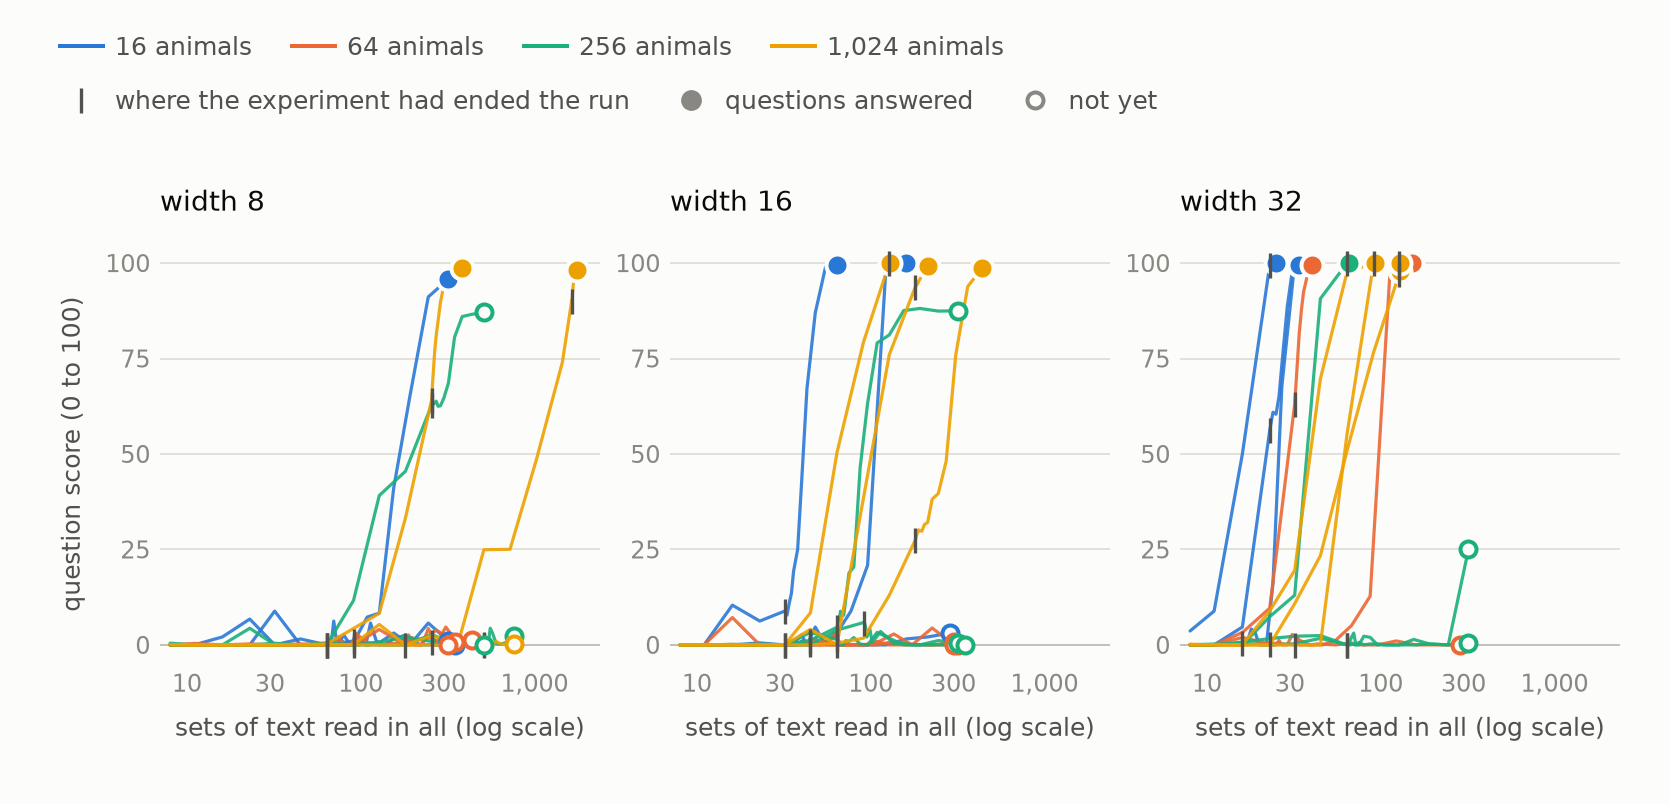
\includegraphics[width=\textwidth]{figures/q_course_equal.png}
\caption{The question score of each first-round model against all the sets it has read: its
original run, then the extra training. The small tick on each line marks where the experiment
had ended the run. Lines that stay on the floor are models still flipping a coin.}
\label{fig:course}
\end{figure}

\subsection*{The unequal-use round}

\begin{table}[H]
\centering\small
\begin{tabular}{@{}rrcccccc@{}}
\toprule
 & & At the start & \multicolumn{5}{c}{After this many more sets} \\
Width & Animals & & 16 & 32 & 64 & 128 & 256 \\
\midrule
8 & 16 & 0, 5, 5 & 0, 1, 0 & 14, 2, 0 & 61, 34, 4 & 84, 93, 69 & 90, 99, 100 \\
8 & 64 & 2, 2, 69 & 5, 1, 69 & 7, 0, 68 & 0, 0, 69 & 0, 0, 77 & 2, 4, 85 \\
8 & 256 & 1, 5, 0 & 0, 21, 0 & 0, 39, 0 & 0, 52, 1 & 0, 63, 0 & 0, 67, 0 \\
8 & 1{,}024 & 1, 0, 25 & 0, 2, 28 & 0, 0, 32 & 0, 1, 37 & 0, 25, 47 & 0, 25, 59 \\
\addlinespace[3pt]
16 & 16 & 94, 85, 94 & 97, 99, 99 & 97, 99, 99 & 97, 99, 99 & 97, 99, 99 & 97, 99, 99 \\
16 & 64 & 49, 55, 75 & 81, 96, 97 & 94, 100, 100 & 100, 100, 100 & 100, 100, 100 & 100, 100, 100 \\
16 & 256 & 0, 3, 38 & 23, 0, 75 & 51, 16, 90 & 79, 70, 98 & 99, 100, 99 & 100, 100, 99 \\
16 & 1{,}024 & 0, 99, 99 & 0, 99, 100 & 0, 99, 100 & 3, 99, 100 & 5, 99, 100 & 100, 99, 100 \\
\addlinespace[3pt]
32 & 16 & 84, 71, 94 & 100, 99, 98 & 100, 99, 98 & 100, 99, 98 & 100, 99, 98 & 100, 99, 98 \\
32 & 64 & 83, 0, 74 & 100, 100, 100 & 100, 100, 100 & 100, 100, 100 & 100, 100, 100 & 100, 100, 100 \\
32 & 256 & 5, 41, 100 & 97, 100, 100 & 100, 100, 100 & 100, 100, 100 & 100, 100, 100 & 100, 100, 100 \\
32 & 1{,}024 & 1, 100, 77 & 84, 100, 99 & 99, 100, 99 & 100, 100, 99 & 100, 100, 99 & 100, 100, 99 \\
\bottomrule
\end{tabular}

\caption{Unequal use. The question score of the three repeats, at the start of the extra
training and after 16 to 256 more sets.}
\label{tab:morezipf}
\end{table}

With unequal use the extra training did much more (table \ref{tab:morezipf}). At the start 7
of the 36 models answered the questions well, 13 were in between and 16 scored under 15.
Afterwards 27 answer well, 4 are in between and 5 score under 15. Every one of the 24 models
of widths 16 and 32 learned the questions, most of them within 64 extra sets. The nine that
did not are all width 8, on 64, 256 and 1,024 animals; on 16 animals all three width-8 models
did learn them.

\subsection*{The 32-bit round}

\begin{table}[H]
\centering\small
\begin{tabular}{@{}rrrrrrrrr@{}}
\toprule
 & & & \multicolumn{4}{c}{Question score} & \multicolumn{2}{c}{Statement score} \\
Animals & Width & Repeat & at the start & after 16 & after 32 & after 64 & at the start & at the end \\
\midrule
16 & 8 & 1 & 0 & 0 & 0 & 0 & 100.0 & 100.0 \\
16 & 8 & 2 & 10 & 17 & 23 & 29 & 100.0 & 100.0 \\
16 & 16 & 1 & 1 & 0 & 0 & 1 & 100.0 & 100.0 \\
16 & 16 & 2 & 80 & 100 & 100 & 100 & 100.0 & 100.0 \\
16 & 32 & 1 & 0 & 1 & 0 & 0 & 100.0 & 100.0 \\
16 & 32 & 2 & 44 & 100 & 100 & 100 & 100.0 & 100.0 \\
256 & 16 & 1 & 0 & 0 & 0 & 0 & 98.6 & 99.7 \\
256 & 16 & 2 & 0 & 0 & 0 & 0 & 99.9 & 100.0 \\
256 & 32 & 1 & 0 & 0 & 0 & 0 & 100.0 & 100.0 \\
\bottomrule
\end{tabular}

\caption{The nine models of the 32-bit round that knew the statements, trained on for 64 more
sets. A set of this round is four times as long, so 64 sets are as much text as 256 sets of
the other rounds.}
\label{tab:morex4}
\end{table}

Here more training changed little (table \ref{tab:morex4}). The two models that were already
part of the way learned the questions within 16 sets. One crept from 10 to 29. The other six
stayed at 0, among them all three on 256 animals. Their statements were untouched.

\subsection*{Across the rounds}

\textbf{Width matters most.} Over the two planned rounds together, the questions are answered
after the extra training by 6 of the 24 models of width 8, 17 of 24 at width 16 and 21 of 24
at width 32.

\textbf{The vocabulary matters with equal use, and hardly at all with unequal use.} You
noticed that the larger vocabulary seemed to do better. With equal use it does, but so does
the smallest: the questions are answered by 6 of the 9 models on 16 animals, 2 of 9 on 64, 1
of 9 on 256 and 8 of 9 on 1,024. With unequal use the figures are 9, 6, 6 and 6 of 9, and all
the failures are width 8.

My first guess about the equal-use pattern was that the 1,024-animal models answer the
questions only because their runs were longer. For widths 16 and 32 that is not it. Their
1,024-animal models answered the questions after 64 to 362 sets in all. Their 64-animal models
that still score 0 or 1 have now read 288 to 320 sets in all, and nothing has moved. For width
8 the matter is open: its 1,024-animal models needed 301 and 1,639 sets, and its 64-animal
models have read 320 to 437.

\section{Is continuing a saved model the same as never stopping?}\label{sec:exact}

A run made again with the same starting numbers, on the same number of processor cores,
repeats the original step for step. So for three of the first-round models I made the original
run again and simply let it go on to 320 sets. Table \ref{tab:exact} sets these beside the same
three models continued from their saved state.

\begin{table}[H]
\centering\small
\begin{tabular}{@{}lrcccc@{}}
\toprule
 & Stopped & \multicolumn{2}{c}{Never stopped} & \multicolumn{2}{c}{Continued from the saved model} \\
Model & at set & at set 128 & at set 320 & at set 128 & at set 320 \\
\midrule
width 8, 16 animals & 64 & 4 & 98 & 8 & 96 \\
width 16, 64 animals & 64 & 0 & 0 & 0 & 0 \\
width 32, 256 animals & 64 & 25 & 62 & 0 & 25 \\
\bottomrule
\end{tabular}

\caption{Question scores of three models, trained without ever being stopped and continued
from the saved model.}
\label{tab:exact}
\end{table}

In two of the three models, stopping and continuing made no real difference. In the third the
continued copy was later: it reached 25 only at set 320, where the run that was never stopped
had 25 at set 128 and 62 at set 320. So the continued models behave in the same way as runs
that were never stopped, but some may be later than they would have been. Three cases are too
few to say how often.

\section{What I make of it}

\textbf{Having a fact and being able to use it are two things.} The report's score asks for a
fact in the one form it was mostly taught in. These models can have every fact in that form
and still be unable to say whether a fox is green. That is worth keeping in mind for your
idea: how much a model ``knows'' depends on how it is asked.

\textbf{Width, and your idea.} Wider models learn the questions more often, as wider models
did better throughout the report. That supports the half of your idea which says that a bigger
model does better. It does not show the other half, that more words overload a model of the
same size: with equal use the largest vocabulary did at least as well as any other at every
width. And it does not look
like a matter of room. Width 8 on 16 animals has almost nothing to hold, and with equal use
two of its three models still cannot answer the questions.

\textbf{A store, and a way of asking it.} This morning you put your idea a second way: a model
is not only a store of what words mean but a way of querying that meaning. These results split
along exactly that line. The store was there: the facts were in the models, and the report
found them in the rows of the word table. What was missing was the querying, the part that
turns a stored fact into the answer to a particular question. That is also the part that was
slow, depended on luck and gained most from width.

\textbf{Unequal use, and a guess about why it helps.} Unequal use made the statements quicker
to learn in the report, and it does the same for the questions. With unequal use a model meets
a few animals constantly. My guess is that those give it an easy place to work out how a
question is answered, and that the way of answering then carries over to the rarer animals.
The review of the research that you asked for points the same way: its first remedy for long
stand-stills was to reshape the text, and unequal use was one of the ways named.

\textbf{The equal-use vocabularies, a second guess.} There are two ways to get the questions
right. One is to learn each question by heart. With 16 animals that is feasible: there are
only 256 different questions, and one set shows each of them 64 to 192 times. The other is to
learn the rule: look up the animal's fact and compare it with the value in the question. With
1,024 animals learning by heart is hopeless (16,384 questions, each shown once to three times
in a set), so the rule is the only way forward. With 64 and 256 animals neither way is easy. I
have not tested this. It fits only half of your impression that variety helps: the most varied
text did best, but the most repeated text did nearly as well, and the two in the middle did
worst.

\textbf{About reinforcement learning.} Ordinary training already rewards the right yes or no,
because the answer is written after every question. What is small is the share of the training
that is about it: 4 sentences in 10 are questions, and only their last word carries the
answer. Training for a while on questions alone would be the direct way to put more weight
there.

\section{Limits, and what is left}

\begin{itemize}
\item \textbf{Nothing here is a test on new sentences.} With equal use a set is the same
      collection of sentences as the set before, in a new order. With unequal use the sets
      are nearly the same: the common sentences are in every set, and the rare ones come up
      in some sets and not in others. Either way, every statement and every question the
      models are graded on was in their training text many times, and I cannot tell a model
      that has learned the rule from one that has learned its questions by heart.
\item \textbf{Whether the skill can appear by itself was not tested,} and cannot be with
      these models, as you pointed out. A design that could test it: give every animal its
      statements, give only some of the animals their questions, and then ask the questions
      about the other animals.
\item \textbf{``Not yet'' is not ``never''.} The models still flipping a coin had 256 more
      sets. This experiment has shown several times that a stand-still can end later.
\item \textbf{Three repeats} are few for something this dependent on chance.
\item \textbf{Still running.} As you asked, the runs of the 32-bit round that ran out of time
      are being trained on now, and the languages of that round that were never run come
      after them. Those results will be reported separately.
\end{itemize}

\textbf{Where everything is.} \s{questions.py} tests saved models on the questions, and
\s{more\_training.py} continues the training of a saved model. Two reviewers checked both
programs and found nothing that makes a number wrong, and a separate measurement of four
models, written without either program, gave the same scores. The scores as the experiment
left them are in \s{results/questions\_now.json}, the continued models in \s{runs\_more}, the
three runs that were never stopped in \s{runs\_more\_exact}. The review of the research on
long stand-stills that you asked for is in \s{results/literature\_stalls.md}.
